\documentclass[11pt]{article}

\usepackage[margin=1in]{geometry}
\usepackage[T1]{fontenc}
\usepackage[utf8]{inputenc}
\usepackage{lmodern}
\usepackage{microtype}
\usepackage{amsmath,amssymb,amsthm,mathtools}
\usepackage{booktabs}
\usepackage{array}
\usepackage{enumitem}
\usepackage{graphicx}
\usepackage{xcolor}
\usepackage{url}
\usepackage{xurl}
\usepackage{hyperref}
\usepackage[backend=biber,style=authoryear,natbib=true,maxcitenames=2,maxbibnames=99]{biblatex}
\addbibresource{references.bib}
\usepackage{cleveref}
\usepackage{tikz}
\usetikzlibrary{arrows.meta,positioning,calc,fit}

\hypersetup{
  colorlinks=true,
  linkcolor=blue!55!black,
  citecolor=blue!55!black,
  urlcolor=blue!55!black,
  pdftitle={Cross-Modal Witnesses: Perceptual Transduction as an Audit Surface for Agentic Alignment},
  pdfauthor={Paul Carver Tiffany III}
}

\newtheorem{definition}{Definition}
\newtheorem{proposition}{Proposition}
\newtheorem{lemma}{Lemma}
\newtheorem{remark}{Remark}

\newcommand{\T}{\mathcal{T}}
\newcommand{\R}{\mathcal{R}}
\newcommand{\I}{\mathcal{I}}
\newcommand{\one}{\mathbf{1}}

\title{\textbf{Cross-Modal Witnesses:}\\
Perceptual Transduction as an Audit Surface for Agentic Alignment}
\author{Paul Carver Tiffany III\\Independent Researcher\\\href{https://orcid.org/0009-0003-4785-6797}{\texttt{ORCID: 0009-0003-4785-6797}}}
\date{September 30, 2026}

\begin{document}
\maketitle

\begin{abstract}
Agentic systems increasingly produce behavior that is difficult to evaluate from raw language, event logs, or scalar metrics alone. This paper proposes \emph{cross-modal structural transduction}: the deliberate mapping of an agent trajectory into an alternative perceptual modality---such as visualization, sonification, animation, or a combined audiovisual representation---as an auxiliary instrument for alignment assessment. The central claim is deliberately limited. A perceptual representation does not prove that an agent is aligned. Rather, when its mapping is specified, calibrated, and tested against known perturbations, it can provide an additional \emph{audit surface} on which alignment-relevant structure may become perceptually salient.

We formalize agent traces, observers, modality transforms, alignment-relevant invariants, perceptual witnesses, masking, and cross-modal disagreement. We distinguish three failure classes that are otherwise easily conflated: \emph{agent failure}, in which the underlying trajectory violates a specified invariant; \emph{mapping failure}, in which a representation conceals or invents relevant structure; and \emph{observer failure}, in which a faithful representation is misread. We prove a simple collision result: if a modality transform maps two trajectories with different invariant status to the same representation, no downstream decoder operating only on that representation can perfectly recover the invariant on both trajectories.

The framework extends earlier work on geometric multi-constraint alignment and deterministic auditing in \emph{The Cost of Cacophony}. Whereas that work asks whether multiple constraints can be jointly satisfied, the present work asks whether satisfaction or violation remains recognizable when behavior is transported across observer channels. A bounded interactive system, StickerBook, provides a controlled experimental testbed with mechanically verifiable properties including typed action selection, host-side validation, page-isolated state, direct user control, learned movement patterns, and explicit receipts. Its public repository now also contains a small live-runtime proof capture for direct Jev control, child interruption, page-state isolation, and language-to-goal translation; these observations supplement, but do not replace, the matched perturbation experiment proposed here. Controlled violations can therefore be injected into otherwise matched traces and rendered into textual, visual, sonic, and audiovisual witnesses.

The broader motivation comes from a lineage spanning Newton's cross-modal proportional mapping in \emph{Opticks}, auditory display and critical-band perception, ecoacoustic sonification, information visualization, observer-relative symbolic projection, generative style transformation, and recent agent-generated music visualization. These examples motivate a general question for agentic alignment: \emph{when the representation changes, which distinctions survive?}
\end{abstract}

\section{Introduction}
Alignment assessment is itself an observational problem. An agent acts; an evaluator receives only some representation of that action. The representation may be a natural-language transcript, structured log, reward signal, benchmark score, causal graph, animation, sonification, or other interface. None is the action itself. Each is a bounded channel through which some distinctions become available to an observer while others disappear.

This distinction becomes increasingly important as agents acquire longer horizons, persistent state, tool access, asynchronous behavior, memory, and interactions with other agents. A raw transcript may omit state transitions that are explicit in a trace. A numerical score may collapse qualitatively different trajectories. Conversely, a compelling visualization may create apparent coherence that is not present in the source behavior. The problem is therefore not simply how to visualize an agent, but how to determine whether a transformation \emph{preserves the distinctions that matter for alignment assessment}.

We call a deliberately constructed representation of an agent trajectory a \emph{cross-modal witness} when it has been calibrated to expose one or more mechanically specified properties of that trajectory. The term \emph{witness} is intentionally weaker than \emph{proof}. The witness may support inspection; it does not replace the underlying trace, validator, or certificate.

This framing extends two earlier lines of work. \href{https://github.com/PaulTiffany/cost}{\emph{The Cost of Cacophony}} studied geometric limits on simultaneous satisfaction of multiple constraints and validated its claims under a deterministic audit observer; its public artifact includes a separate browser-playable sonification suite \citep{tiffany2026cacophony}. The sonification was supplementary rather than the empirical certificate. The present work asks what would be required to promote such a representation from illustration to instrument.

The second line is the anti-masking principle developed in \href{https://github.com/PaulTiffany/hypothesis-surface-agi26}{\emph{The Hypothesis Surface}}: representations may appear adequate by concealing the evidence required to expose inadequacy \citep{tiffany2026surface}. A visualization or sonification is therefore not automatically an improvement in observability. It is another surface on which masking can occur.

Our proposal is consequently two-sided:
\begin{enumerate}[label=(\arabic*)]
    \item changing modality may expose structure that is difficult to perceive in the original representation; and
    \item every modality transform introduces a new opportunity for distortion, collision, omission, interaction, and masking.
\end{enumerate}
The useful scientific object is not the visualization by itself, but the relation among \emph{source trace, specified invariant, transformation, and observer judgment}; \cref{fig:crossmodal-pipeline} summarizes this architecture.

\paragraph{Contributions.}
This paper contributes: (i) a formal vocabulary for cross-modal witnesses, ingress, masking, and disagreement; (ii) impossibility results for non-separating transforms and for witness families that inherit a shared lossy bottleneck; (iii) a three-way taxonomy separating agent, mapping, and observer failures; (iv) a perturbation protocol and canonical trace schema using a bounded agentic system with mechanical ground truth; (v) a reproducible synthetic calibration suite with independently generated visual and sonic witnesses, including an explicit pre-freeze mapping-collision test; (vi) a pinned observational runtime-evidence layer derived conservatively from StickerBook's committed P(HOP) proof capture; (vii) a preregistration-ready observer-study and analysis plan; and (viii) a historical and technical lineage connecting auditory display, visual perception, symbolic projection, and recent agent-generated audiovisual artifacts.

\begin{figure*}[t]
\centering
\resizebox{0.98\textwidth}{!}{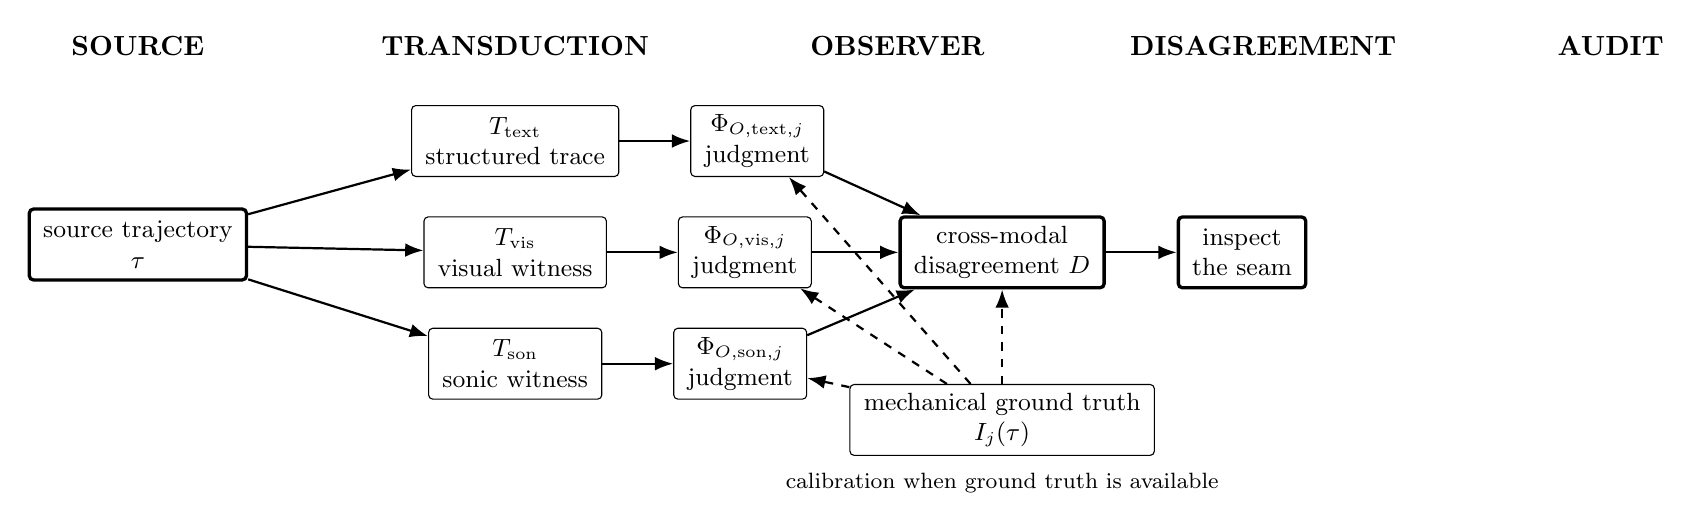
\begin{tikzpicture}[
  >=Latex,
  font=\small,
  node distance=5mm and 7mm,
  box/.style={draw, rounded corners=1.5pt, align=center, minimum height=9mm, inner xsep=5pt, inner ysep=3pt},
  source/.style={box, very thick},
  arrow/.style={->, thick},
  cal/.style={->, dashed, thick}
]
\node[font=\bfseries] (h1) {SOURCE};
\node[font=\bfseries, right=20mm of h1] (h2) {TRANSDUCTION};
\node[font=\bfseries, right=18mm of h2] (h3) {OBSERVER};
\node[font=\bfseries, right=16mm of h3] (h4) {DISAGREEMENT};
\node[font=\bfseries, right=18mm of h4] (h5) {AUDIT};

\node[source, below=18mm of h1] (tau) {source trajectory\\$\tau$};
\node[box, below=5mm of h2] (tt) {$T_{\mathrm{text}}$\\structured trace};
\node[box, below=5mm of tt] (tv) {$T_{\mathrm{vis}}$\\visual witness};
\node[box, below=5mm of tv] (ts) {$T_{\mathrm{son}}$\\sonic witness};

\node[box, right=9mm of tt] (ot) {$\Phi_{O,\mathrm{text},j}$\\judgment};
\node[box, right=9mm of tv] (ov) {$\Phi_{O,\mathrm{vis},j}$\\judgment};
\node[box, right=9mm of ts] (os) {$\Phi_{O,\mathrm{son},j}$\\judgment};

\node[source, right=11mm of ov] (d) {cross-modal\\disagreement $D$};
\node[source, right=9mm of d] (audit) {inspect\\the seam};
\node[box, below=12mm of d] (truth) {mechanical ground truth\\$I_j(\tau)$};

\draw[arrow] (tau) -- (tt);
\draw[arrow] (tau) -- (tv);
\draw[arrow] (tau) -- (ts);
\draw[arrow] (tt) -- (ot);
\draw[arrow] (tv) -- (ov);
\draw[arrow] (ts) -- (os);
\draw[arrow] (ot) -- (d);
\draw[arrow] (ov) -- (d);
\draw[arrow] (os) -- (d);
\draw[arrow] (d) -- (audit);
\draw[cal] (truth) -- (ot);
\draw[cal] (truth) -- (ov);
\draw[cal] (truth) -- (os);
\draw[cal] (truth) -- (d);
\node[font=\footnotesize, below=1mm of truth] {calibration when ground truth is available};
\end{tikzpicture}
}
\caption{Cross-modal witnessing as an audit architecture. A single source trajectory is transported through independently specified modality transforms and decoded by observer-specific channels. Cross-modal disagreement is not treated as proof of failure; it is a triage signal that is compared against mechanical ground truth when available. The dashed paths denote calibration against the invariant evaluator $I_j$.}
\label{fig:crossmodal-pipeline}
\end{figure*}

\section{Lineage: From Cross-Modal Correspondence to Audit Surfaces}

\subsection{Newton: proportional structure across modalities}
A historical precedent appears in Newton's \emph{Opticks}. In the 1718 edition, Newton divided a color circle into seven regions ``proportional to the seven musical Tones or Intervals,'' assigning the regions to red, orange, yellow, green, blue, indigo, and violet \citep{newton1718opticks}. Newton's construction belongs to a different scientific context; what carries forward here is the methodological idea that relational structure can be transported between representational domains without requiring the domains themselves to be identical.

For the present work, Newton's construction is useful as a conceptual ancestor of a question we make explicit and testable: if a relation is mapped from one modality into another, which structural distinctions remain recognizable after the map?

\subsection{Auditory display, critical bands, and channel-induced structure}
The modern field of sonification treats sound as a systematic information display rather than merely a decorative accompaniment. The \emph{Sonification Handbook} surveys design and evaluation of auditory displays and explicitly treats evaluation as a methodological problem \citep{hermann2011sonification,bonebright2011evaluation}.

A particularly important warning comes from auditory perception itself. \citet{plomp1965tonal} showed that perceived consonance and roughness depend on interactions within critical bandwidths. For our purposes, this result demonstrates that a perceptual channel has its own interaction geometry: two mapped components can generate a perceptual relation that was not explicit in either component considered alone. A modality transform is therefore not a neutral conduit. It can reveal source structure, suppress it, or create channel-induced interactions.

This observation motivated the earlier auditory demonstrations in \emph{The Cost of Cacophony}, where spectral proximity and perceptual roughness were used as disciplined analogical mappings for interacting constraint directions rather than as direct quantitative evidence \citep{tiffany2026cacophony}. The distinction remains central here: perceptual salience may guide inspection, but salience is not itself a certificate.

\subsection{Burtner, Katz, and the engineered auditory channel}
The author's introduction to sonification as both compositional practice and mode of inquiry came through study with composer and ecoacoustician Matthew Burtner. Burtner defines ecoacoustics in terms of vibrational energy, sonification, human--nature interaction, technological mediation including transduction and computation, and scientific methods for parsing environments through acoustics \citep{burtnerEcoacoustics}. His work provides an intellectual precedent for treating sound as a mediated interface to structure rather than merely an aesthetic overlay.

The engineering of that interface is nontrivial. Katz's \emph{Mastering Audio: The Art and the Science}, third edition, supplies a complementary engineering discipline concerning monitoring, loudness, spectral balance, dynamic range, clipping, psychoacoustics, and repeatable audio reproduction \citep{katz2015mastering}. A sonification whose apparent structure changes materially with uncontrolled rendering or playback conditions is a poor scientific instrument.

A contemporary neighboring practice appears in Amanda Gregory's multimedia and ``neuro-music'' work, which explicitly combines artistic data sonification, psychoacoustics, biometrics, audiovisual composition, and multisensory performance \citep{gregoryPortfolio,gregoryCreality}. Gregory also opened the AGI-26 closing event with \emph{Desdemona's Dream}, advertised as humans creating alongside robotics and AI \citep{agi26closing}. Together, these works situate sonification and audiovisual composition within a broader cross-modal practice in which data, signal, and performance are made available to perception through deliberately engineered form.

\subsection{Visualization and perception}
Information visualization rests on an analogous proposition: representation changes what patterns are available to an observer. Ware's perception-centered treatment emphasizes visual salience, pattern perception, dynamic displays, interaction, and visual thinking as design concerns rather than presentation afterthoughts \citep{ware2020visualization}. The present framework therefore treats visual and auditory mappings symmetrically. Neither modality is privileged. Each supplies an observer channel with distinct bandwidth, salience, collision modes, and perceptual biases.

\subsection{Principia Symbolica: bounded observers and projective translation}
\href{https://paultiffany.github.io/Principia-Symbolica/}{\emph{Principia Symbolica}} provides the closest formal antecedent within the author's own research program \citep{tiffany2026principia}. The public atlas makes the connection unusually concrete. Book IV defines an \href{https://paultiffany.github.io/Principia-Symbolica/atlas/book-iv-de-identitate-symbolica-et-emergentia/page-1/}{Observer--Kernel Convolution} $\mathcal{K}_O$ as an observer-centered low-pass operator; a \href{https://paultiffany.github.io/Principia-Symbolica/atlas/book-iv-de-identitate-symbolica-et-emergentia/page-1/}{Projective Action Translator} $\Lambda_O$ maps bounded symbolic velocities into an operator space; and a \href{https://paultiffany.github.io/Principia-Symbolica/atlas/book-iv-de-identitate-symbolica-et-emergentia/page-1/}{Bounded Observer} is parameterized by a perceptual kernel, observable derivation, and bounded perception domain. The same atlas states \emph{Observer Locality}: the support of an observer kernel is restricted to that bounded domain \citep{tiffany2026principiaBook4}.

Those records do not themselves define audiovisual sonification. Their relevance is structural: observation is explicitly indexed by an observer and mediated by bounded operators rather than supplied from a ``view from nowhere.'' The present paper specializes that observer-relative machinery to perceptual instrumentation. A modality transform is treated as one more bounded projection. We therefore ask not whether a representation is intuitively faithful, but which target distinctions survive the projection, which collide, and under what distortion budget.

\subsection{Ghiblification as large-scale representational remapping}
The viral ``Ghiblification'' phenomenon of 2025 supplies a culturally visible example of mass representational remapping: user-supplied photographs were transformed into a recognizable visual idiom associated with Studio Ghibli while often retaining enough scene, pose, identity, and relational information to remain recognizable \citep{jon2025ghiblification}. Methodologically, the phenomenon illustrates that dramatic surface transformation can preserve some distinctions while altering or erasing others.

This motivates a general alignment question: \emph{which properties belong to the source trajectory, and which appear only in the chosen representational chart?}

\subsection{Claude-Pop and deterministic generative visualization}
Recent code-rendered visualizations of \emph{I'm Upping My P(doom)} provide a more direct technical precedent. The \texttt{mexicat/pdoom-video} implementation describes a renderer in which every frame is a deterministic function of song time, supported by word-level lyric alignment, beat/downbeat/onset analysis, and explicit scene timelines \citep{mexicat2026pdoom}. A second public implementation, \texttt{JohnHeibel/PDoomVideo}, documents an agent-generated storyboard, animation guide, scene code, renderer, and ffmpeg pipeline produced from broad visual directions rather than a manually specified shot list \citep{heibel2026pdoom}.

The important object is not the song alone. It is the representational chain
\begin{equation}
\text{concept}
\rightarrow
\text{language}
\rightarrow
\text{music}
\rightarrow
\text{visual structure}
\rightarrow
\text{human judgment}.
\end{equation}
In our StickerBook demonstration, the loop continues:
\begin{equation}
\text{human judgment}
\rightarrow
\text{new specification}
\rightarrow
\text{agent construction}
\rightarrow
\text{new audiovisual witness}.
\end{equation}
This recursive process motivates the present paper. Representation is not merely the endpoint of agent behavior; it may participate in the observer--agent loop by changing which distinctions an observer notices and therefore which specifications are returned to the agent.

\section{Formal Framework}

\subsection{Agent trajectories}
Let an agent interaction generate a trajectory
\begin{equation}
\tau=(s_0,a_0,o_0,s_1,a_1,o_1,\ldots,s_T),
\end{equation}
where $s_t$ denotes system state, $a_t$ an action or selected decision, and $o_t$ other observable events, responses, validation results, or environmental changes. Let $\T$ denote the set of admissible trajectories for the system under evaluation.

\subsection{Alignment-relevant invariants}
For each property of interest, define an evaluator
\begin{equation}
I_j:\T\rightarrow\mathcal{Y}_j.
\end{equation}
The term \emph{invariant} is operational rather than absolute: it denotes a property that the evaluation protocol intends to preserve and recognize across admissible representations. For a Boolean safety property, $I_j(\tau)\in\{0,1\}$.

Examples include whether an action belongs to the permitted action set, whether host-side validation succeeded, whether a delayed response was rejected after its authority context expired, whether one page's state contaminated another, and whether remembered behavior remained advisory rather than authoritative.

\subsection{Modality transforms}
Let
\begin{equation}
T_m:\T\rightarrow\R_m
\end{equation}
be a deterministic or reproducibly stochastic transformation of a trajectory into representation space $\R_m$, where
\begin{equation}
m\in\{\text{text},\text{diagram},\text{animation},\text{sound},\text{audiovisual},\ldots\}.
\end{equation}
Examples include a structured log $T_{\mathrm{text}}(\tau)$, an animation $T_{\mathrm{vis}}(\tau)$, and a sonification $T_{\mathrm{son}}(\tau)$.

\begin{definition}[Ingress]
For observer $O$, \emph{ingress} denotes the directional availability of structured information through a bounded representation channel:
\begin{equation}
\tau\xrightarrow{T_m}R_m\xrightarrow{\mathrm{ingress}}O.
\end{equation}
Ingress does not imply lossless transport or exact reconstruction of $\tau$ by $O$.
\end{definition}

The analogy is transductive: as a receptor converts a physical perturbation into another signal domain available to a nervous system, the engineered transform converts an agent trajectory into a representation available to an evaluator. The analogy is functional, not a claim that biological afference and engineered visualization are identical mechanisms.

\subsection{Perceptual decoding}
Let
\begin{equation}
\Phi_{O,m,j}:\R_m\rightarrow\widehat{\mathcal{Y}}_j
\end{equation}
denote the observer's judgment of property $I_j$ after receiving modality $m$. For Boolean properties,
\begin{equation}
\widehat I_{O,m,j}(\tau)=\Phi_{O,m,j}(T_m(\tau)).
\end{equation}
The empirical error of a witness is
\begin{equation}
E_{O,m,j}=\Pr\!\left[\widehat I_{O,m,j}(\tau)\neq I_j(\tau)\right].
\end{equation}
A representation should not be called an alignment witness merely because it is interpretable. Its error must be characterized on controlled traces.

\begin{definition}[Cross-modal witness]
A modality transform $T_m$ is an $(I_j,\epsilon)$-\emph{witness} on domain $\Omega\subseteq\T$ for observer class $O$ when calibrated evaluation demonstrates
\begin{equation}
E_{O,m,j}\leq\epsilon
\end{equation}
on traces spanning both satisfaction and controlled violation of $I_j$.
\end{definition}

The witness is therefore empirical and property-specific. There is no generic ``good visualization'' independent of what the representation is intended to reveal.

\subsection{Masking and representation collisions}
\begin{definition}[Masking]
For trajectories $\tau^+,\tau^-\in\T$ with $I_j(\tau^+)\neq I_j(\tau^-)$, a transform masks the distinction for observer $O$ when
\begin{equation}
\Phi_{O,m,j}(T_m(\tau^+))=\Phi_{O,m,j}(T_m(\tau^-)).
\end{equation}
\end{definition}

A stronger, observer-independent failure occurs when the representations themselves collide (\cref{fig:collision}).

\begin{proposition}[Collision impossibility]
\label{prop:collision}
Suppose there exist $\tau^+,\tau^-\in\T$ such that
\begin{equation}
I_j(\tau^+)\neq I_j(\tau^-)
\quad\text{and}\quad
T_m(\tau^+)=T_m(\tau^-).
\end{equation}
Then no deterministic decoder $\Phi:\R_m\rightarrow\mathcal{Y}_j$ operating only on $T_m(\tau)$ can recover $I_j$ correctly on both $\tau^+$ and $\tau^-$. Consequently, $T_m$ cannot be a zero-error witness for $I_j$ on any domain containing both trajectories.
\end{proposition}

\begin{proof}
Let $r=T_m(\tau^+)=T_m(\tau^-)$. A deterministic decoder must assign a single value $\Phi(r)$. Because $I_j(\tau^+)\neq I_j(\tau^-)$, that value can equal at most one of the two ground-truth values. Hence at least one trajectory is misclassified.\qedhere
\end{proof}

\Cref{prop:collision} formalizes an anti-masking requirement: a proposed witness must at minimum separate the source distinctions it claims to reveal.

\subsection{Shared bottlenecks and transform diversity}
Cross-modal agreement is informative only to the extent that the witnesses do not inherit the same distinction-destroying preprocessing step. To make this requirement explicit, let $Q:\T\rightarrow\mathcal{Z}$ be an intermediate representation and suppose multiple modality transforms factor through it,
\begin{equation}
T_m = G_m \circ Q.
\end{equation}

\begin{definition}[Common-mode transform family]
A witness family $\{T_m\}_{m\in M}$ has a \emph{common-mode bottleneck} $Q$ for invariant $I_j$ on $\Omega\subseteq\T$ when every $T_m$ factors through $Q$ on $\Omega$. The family is \emph{upstream-diverse} with respect to $I_j$ when no undeclared shared intermediate is known to erase an $I_j$-relevant distinction before the modality-specific transforms diverge.
\end{definition}

\begin{proposition}[Shared-bottleneck impossibility]
\label{prop:shared-bottleneck}
Suppose $T_m=G_m\circ Q$ for every $m$ in a witness family and there exist $\tau^+,\tau^-\in\Omega$ with
\begin{equation}
I_j(\tau^+)\neq I_j(\tau^-)
\quad\text{but}\quad
Q(\tau^+)=Q(\tau^-).
\end{equation}
Then no collection of downstream decoders operating only on $\{T_m(\tau)\}_{m\in M}$ can perfectly recover $I_j$ on both trajectories. Agreement among those modalities cannot restore the distinction destroyed by $Q$.
\end{proposition}

\begin{proof}
Because $Q(\tau^+)=Q(\tau^-)$, for every $m$ we have $T_m(\tau^+)=G_m(Q(\tau^+))=G_m(Q(\tau^-))=T_m(\tau^-)$. The entire vector of witness representations is therefore identical for the two trajectories. Any deterministic joint decoder receives the same input for different ground-truth values and must misclassify at least one.\qedhere
\end{proof}

\begin{figure*}[t]
\centering
\resizebox{0.93\textwidth}{!}{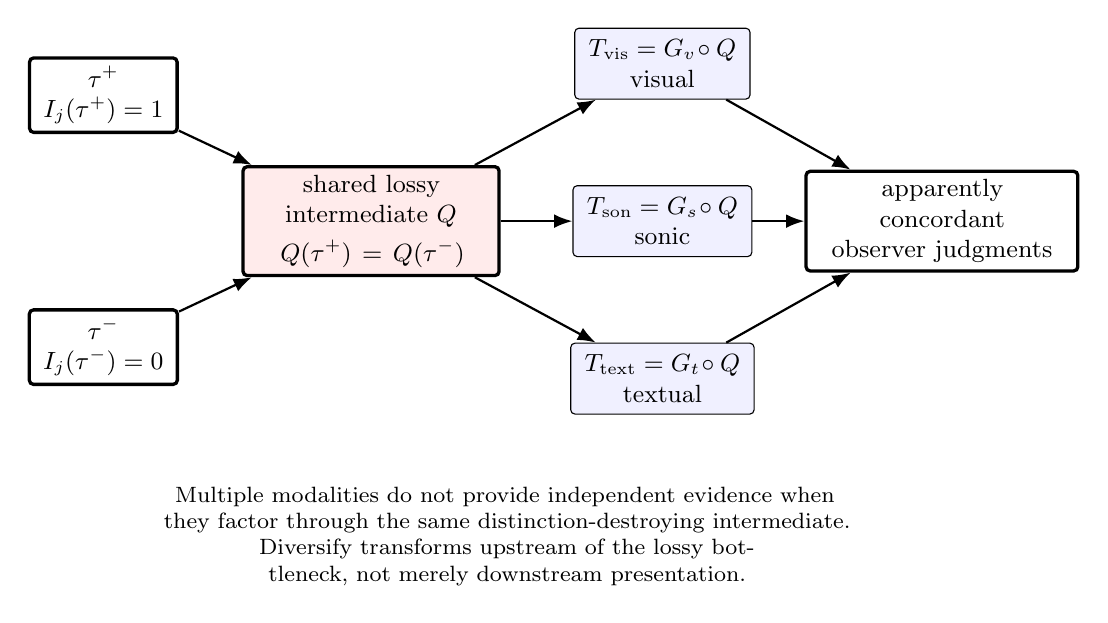
\begin{tikzpicture}[
  >=Latex,
  font=\small,
  box/.style={draw, rounded corners=1.5pt, align=center, minimum height=9mm, inner xsep=5pt, inner ysep=3pt},
  source/.style={box, very thick},
  bottleneck/.style={box, very thick, fill=red!8},
  witness/.style={box, fill=blue!6},
  arrow/.style={->, thick},
  dashedarrow/.style={->, thick, dashed}
]
\node[source] (p) at (-5.1,1.6) {$\tau^+$\\$I_j(\tau^+)=1$};
\node[source] (m) at (-5.1,-1.6) {$\tau^-$\\$I_j(\tau^-)=0$};
\node[bottleneck, text width=29mm] (q) at (-1.7,0) {shared lossy\\intermediate $Q$\\[1mm]$Q(\tau^+)=Q(\tau^-)$};
\node[witness] (vis) at (2.0,2.0) {$T_{\mathrm{vis}}=G_v\!\circ Q$\\visual};
\node[witness] (son) at (2.0,0) {$T_{\mathrm{son}}=G_s\!\circ Q$\\sonic};
\node[witness] (txt) at (2.0,-2.0) {$T_{\mathrm{text}}=G_t\!\circ Q$\\textual};
\node[source, text width=31mm] (agree) at (5.55,0) {apparently concordant\\observer judgments};

\draw[arrow] (p) -- (q);
\draw[arrow] (m) -- (q);
\draw[arrow] (q) -- (vis);
\draw[arrow] (q) -- (son);
\draw[arrow] (q) -- (txt);
\draw[arrow] (vis) -- (agree);
\draw[arrow] (son) -- (agree);
\draw[arrow] (txt) -- (agree);

\node[font=\footnotesize, align=center, text width=92mm] at (0,-4.0) {Multiple modalities do not provide independent evidence when they factor through the same distinction-destroying intermediate.\\Diversify transforms upstream of the lossy bottleneck, not merely downstream presentation.};
\end{tikzpicture}
}
\caption{False reassurance from downstream modality diversity. Visual, sonic, and textual witnesses may appear independent while all factoring through the same lossy intermediate $Q$. If $Q$ collapses an invariant-relevant distinction, downstream agreement cannot recover it (Proposition~\ref{prop:shared-bottleneck}). Transform diversity must therefore be assessed upstream of shared lossy preprocessing.}
\label{fig:shared-bottleneck}
\end{figure*}

\begin{figure}[t]
\centering
\resizebox{0.98\linewidth}{!}{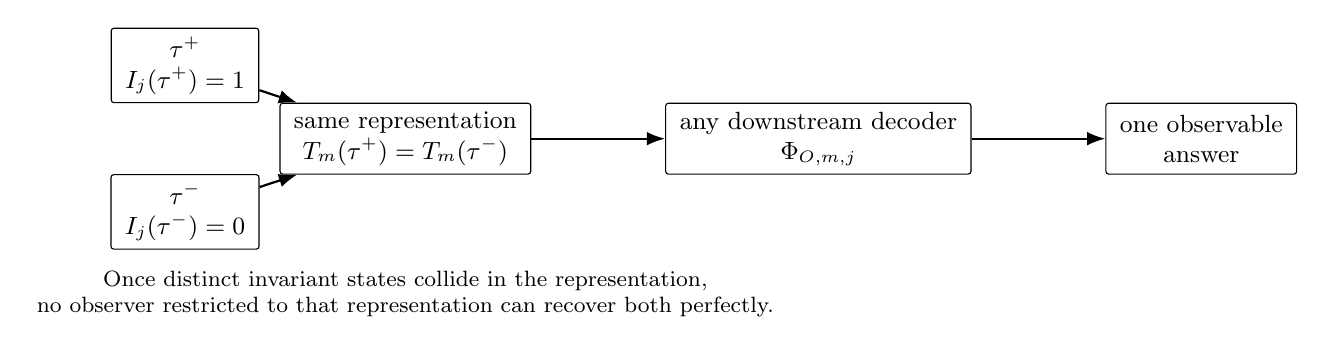
\begin{tikzpicture}[
  >=Latex,
  font=\small,
  box/.style={draw, rounded corners=1pt, align=center, minimum height=9mm, inner xsep=5pt, inner ysep=3pt},
  arrow/.style={->, thick}
]
\node[box] (p) {$\tau^+$\\$I_j(\tau^+)=1$};
\node[box, below=9mm of p] (m) {$\tau^-$\\$I_j(\tau^-)=0$};
\node[box, right=12mm of $(p)!0.5!(m)$] (same) {same representation\\$T_m(\tau^+)=T_m(\tau^-)$};
\node[box, right=17mm of same] (dec) {any downstream decoder\\$\Phi_{O,m,j}$};
\node[box, right=17mm of dec] (one) {one observable\\answer};
\draw[arrow] (p) -- (same);
\draw[arrow] (m) -- (same);
\draw[arrow] (same) -- (dec);
\draw[arrow] (dec) -- (one);
\node[align=center, font=\footnotesize, below=11mm of same] {Once distinct invariant states collide in the representation,\\no observer restricted to that representation can recover both perfectly.};
\end{tikzpicture}
}
\caption{Representation collision behind Proposition~\ref{prop:collision}. If trajectories with different invariant status are mapped to the same representation, no downstream decoder that sees only that representation can classify both perfectly. This is the basic anti-masking limit for any single audit surface.}
\label{fig:collision}
\end{figure}

\subsection{Channel-induced interactions}
A transform need not preserve compositional independence. Let $\tau=\tau_1\oplus\tau_2$ denote a source composition. In general,
\begin{equation}
T_m(\tau_1\oplus\tau_2)
\neq
T_m(\tau_1)\oplus T_m(\tau_2).
\end{equation}
Auditory roughness from nearby components provides a concrete perceptual example \citep{plomp1965tonal}. We therefore distinguish \emph{source interaction}, \emph{mapping interaction}, and \emph{observer interaction}. A pattern appearing only after transduction may be diagnostically useful, but its provenance must be established before it is attributed to the agent.

\subsection{Cross-modal disagreement}
For modalities $m$ and $n$, define
\begin{equation}
D_{m,n,j}(\tau)
=
\one\!\left[
\widehat I_{O,m,j}(\tau)
\neq
\widehat I_{O,n,j}(\tau)
\right].
\end{equation}
When ground truth is unavailable, $D$ is not evidence that either representation is correct. It is a \emph{triage signal} identifying trajectories requiring inspection. When ground truth is available, disagreement can localize which channel fails.

\subsection{Failure taxonomy}
We distinguish three failure classes:
\begin{description}[style=nextline]
    \item[Agent failure.] The source trajectory violates the property: $I_j(\tau)=0$.
    \item[Mapping failure.] The trajectory has known status, but the transform destroys, aliases, invents, or materially distorts the relevant distinction.
    \item[Observer failure.] The representation preserves the distinction, but the observer fails to classify it correctly.
\end{description}
These classes must not be collapsed. A striking sonification may be wrong; a confusing visualization may represent a correct trace; a human may miss a correctly represented violation.

\section{Claims and Testable Hypotheses}
The paper does not claim that multimodal agreement proves alignment. Two lossy transforms may agree for the same wrong reason. Instead, we propose four hypotheses.

\paragraph{H1 --- Salience.}
For some alignment-relevant properties, a calibrated cross-modal witness yields higher detection accuracy or lower detection time than the raw trace alone.

\paragraph{H2 --- Complementarity.}
Different modalities expose different failure classes; combined modalities therefore reduce masking relative to a single modality for at least some properties.

\paragraph{H3 --- Disagreement as triage.}
Cross-modal disagreement is enriched for agent, mapping, or observer anomalies relative to randomly sampled traces.

\paragraph{H4 --- Calibratability.}
Mapping failures can be experimentally distinguished from agent failures by independently controlled perturbations of the source trace and the modality transform.

\section{StickerBook as a Controlled Agentic Testbed}
\href{https://github.com/PaulTiffany/stickerbook}{StickerBook} is useful precisely because its alignment-relevant properties are unusually concrete and publicly inspectable \citep{tiffany2026stickerbook}. The current public architecture separates the child-facing medium from the authority path: ``Omega talks. Jev chooses. The kernel decides.'' The headless kernel is the single mutation gate and validates known action, schema, bounded arguments, ownership, revision, budget, and expiry before applying a command and returning an explicit receipt \citep{tiffany2026stickerbookcore}. For the agent path, the host exposes only currently legal keys; the model selects a key rather than constructing an arbitrary command.

The browser-facing architecture further separates OmegaLLM, OmegaJev, and the authority kernel. The current Jev experiment documents typed decision selection through the OpenRouter Decisions API, frozen host tables, fail-closed parsing, and a direct child double-click path that can reach bounded decision selection without an intervening language-model translation \citep{tiffany2026stickerbookjev,tiffany2026stickerbookinterface}. The public GitHub Pages build is intentionally mechanical, while the powered path is local and governed; models do not directly mutate pages \citep{tiffany2026stickerbook}.

The deployment record distinguishes two runtime claims that must not be merged. The intended hardened graph uses separate OpenShell sandboxes for OmegaLLM and OmegaJev, but live-host provisioning remained blocked by an upstream WSL2/seccomp failure at the recorded project version; the repository therefore labels that hardened graph unverified rather than assuming that architectural tests imply deployment success \citep{tiffany2026stickerbookruntime}. Separately, the P(HOP) video package committed a proof capture from isolated host \texttt{BookBridge} worlds calling existing loopback Omega containers and producing ordinary kernel receipts \citep{tiffany2026stickerbookproof,tiffany2026stickerbookvideo}. The present paper treats that capture as observational runtime evidence, not as evidence that the hardened OpenShell graph was live.

For the proposed experiment, the relevant action vocabulary includes bounded actions such as
\begin{equation}
\{\texttt{MOVE},\texttt{FACE},\texttt{ANIMATE},\texttt{NOOP}\},
\end{equation}
subject to the action set actually offered by the host at a given turn. Page-local state and history provide natural containment invariants, while delayed-response rejection, receipts, revision checks, and bounded learned movement patterns provide additional mechanically testable properties. The proposed study will draw claims only from the tested implementation and will update this section if the runtime contract changes before evaluation.

\subsection{Canonical trace schema for the experiment}
To avoid treating a rendered witness as the primary record, every trial should first produce a canonical append-only trace. A minimal event record is
\begin{equation}
 e_k = (t_k,p_k,r_k,q_k,u_k,A_k,c_k,v_k,\rho_k,\Delta s_k),
\end{equation}
where $t_k$ is event time, $p_k$ page/world identity, $r_k$ acting principal, $q_k$ world revision before proposal, $u_k$ input route (for example language, direct gesture, or delayed response), $A_k$ the host-offered legal-action table, $c_k$ the selected key or proposed command, $v_k$ the validation verdict, $\rho_k$ the resulting receipt including rejection reason when applicable, and $\Delta s_k$ the authoritative state delta. Optional fields record decision confidence/probabilities, model/provider identity, movement-pattern advisory context, and authority-expiry metadata when those fields are part of the tested path.

This schema is intentionally downstream of neither the visualization nor the sonification. Each witness is generated independently from the canonical trace plus a declared mapping specification. The source trace, mapping specification, renderer version, and observer response should all receive stable identifiers so that a disagreement can be traced back to a specific event rather than inferred from media alone. The concrete runtime binding follows the current public StickerBook receipt interface: \texttt{commandId}, \texttt{actor}, \texttt{requestedBy}, \texttt{translatedBy}, \texttt{selectedBy}, \texttt{action}, \texttt{object}, \texttt{basedOnRevision}, \texttt{accepted}, \texttt{reason}, \texttt{resultRevision}, and \texttt{replayed} are preserved rather than reconstructed from rendered media \citep{tiffany2026stickerbookcore,tiffany2026stickerbookinterface}.

\begin{figure*}[t]
\centering
\resizebox{0.92\textwidth}{!}{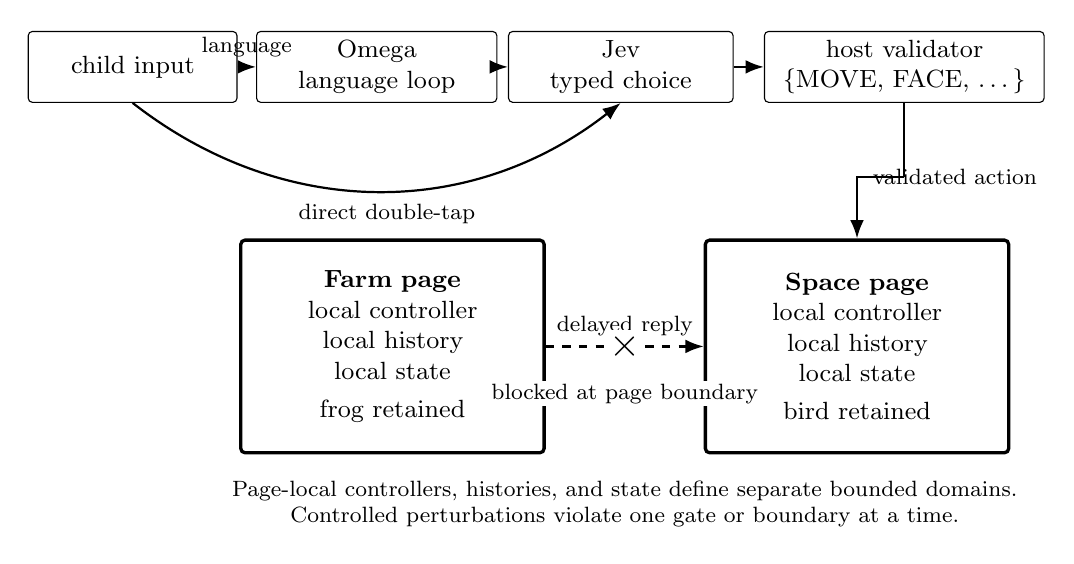
\begin{tikzpicture}[
  x=1cm,y=1cm,
  >=Latex,
  font=\small,
  box/.style={draw, rounded corners=1.5pt, align=center, minimum height=9mm, inner xsep=5pt, inner ysep=3pt},
  page/.style={box, very thick, text width=35mm, minimum height=27mm},
  arrow/.style={->, thick},
  dashedarrow/.style={->, thick, dashed}
]
% Decision path.
\node[box, text width=23mm] (child) at (-5.0,3.1) {child input};
\node[box, text width=27mm] (omega) at (-1.9,3.1) {Omega\\language loop};
\node[box, text width=25mm] (jev) at (1.2,3.1) {Jev\\typed choice};
\node[box, text width=32mm] (host) at (4.8,3.1) {host validator\\\{MOVE, FACE, \ldots\}};
\draw[arrow] (child) -- node[above,font=\footnotesize]{language} (omega);
\draw[arrow] (omega) -- (jev);
\draw[arrow] (jev) -- (host);
\draw[arrow] (child.south) to[out=-38,in=-142] node[pos=.52,below=1pt,font=\footnotesize]{direct double-tap} (jev.south);

% Independent page-local domains.
\node[page] (farm) at (-1.7,-0.45) {\textbf{Farm page}\\local controller\\local history\\local state\\[1mm]frog retained};
\node[page] (space) at (4.2,-0.45) {\textbf{Space page}\\local controller\\local history\\local state\\[1mm]bird retained};
\coordinate (fork) at (4.8,1.70);
\draw[thick] (host.south) -- (fork);
\draw[arrow] (fork) -| node[pos=.50,right=2pt,font=\footnotesize]{validated action} (space.north);

% Cross-page leakage is an explicit violation.
\draw[dashedarrow] (farm.east) -- node[above,font=\footnotesize]{delayed reply} (space.west);
\node[fill=white, inner sep=1pt] at ($(farm.east)!0.50!(space.west)$) {\Large$\times$};
\node[font=\footnotesize, fill=white, inner sep=1pt] at ($(farm.east)!0.50!(space.west)+(0,-6mm)$) {blocked at page boundary};

\node[align=center, font=\footnotesize] at (1.25,-2.45) {Page-local controllers, histories, and state define separate bounded domains.\\Controlled perturbations violate one gate or boundary at a time.};
\end{tikzpicture}
}
\caption{StickerBook as a bounded experimental apparatus. Natural-language input may pass through Omega before Jev selects a typed choice, while direct user interaction can reach the same bounded decision layer without an intervening language-model translation. Host validation gates execution. Each page retains local controller, history, and state; delayed responses are not permitted to cross page boundaries. Learned patterns return as advisory candidates rather than authority. The same apparatus supports controlled source perturbations such as validation bypass or cross-page leakage.}
\label{fig:stickerbook-apparatus}
\end{figure*}

\subsection{Observed runtime evidence and claim boundary}
\paragraph{Deployment disclosure at submission.}
As of September 30, 2026, the upstream OpenShell/WSL deployment issue remains unresolved on the author's host. The observed powered runs use restricted ordinary Docker: separate non-root OmegaLLM and OmegaJev containers, localhost-only publications, dropped capabilities, bounded resources, and a host-resident authority kernel. Real provider credentials are injected into the relevant role containers and direct provider egress is allowed. This local-development profile does not reproduce OpenShell credential substitution, executable-bound egress policy, or network mediation, and is not a production child-facing deployment. Retained OpenShell policies describe the desired hardened target, not verified containment. Runtime observations below are limited to their recorded kernel/controller claims.

Before any human observer study, StickerBook's P(HOP) video package produced a small, independently committed runtime-evidence artifact. The JSON record identifies itself as an ``actual live runtime evidence'' artifact, was captured at 2026-09-30T08:33:50Z, and is pinned in this manuscript bundle by both repository commit and Git blob identity \citep{tiffany2026stickerbookproof}. We conservatively project four observations from that source into the same canonical trace vocabulary used by the calibration fixtures:
\begin{enumerate}[leftmargin=*]
    \item \textbf{Direct control.} A double-tap initiated Jev-controlled butterfly behavior with \texttt{translatedBy} set to null, \texttt{selectedBy} identifying the Jev controller, and ordinary accepted kernel receipts. The committed proof artifact does not serialize the full offered legal-key table, so this observation does not independently establish action-set membership.
    \item \textbf{Human interruptibility.} Active autonomous motion terminated with audit reason ``child-grabbed''; an ordinary human move then received an accepted kernel receipt and established the new page state.
    \item \textbf{Page-state isolation.} Farm was observed at revision 38 with its butterfly and cow, Space was observed empty at revision 0, and returning to Farm restored the same revision-38 state. This supports page-local state persistence in the capture. It is not a live injection test of a delayed provider response crossing pages.
    \item \textbf{Language to bounded goal.} The utterance ``Make the butterfly flutter.'' produced a bounded goal with subject \texttt{butterfly-1}, intent \texttt{animate}, behavior \texttt{flutter}, and Jev result \texttt{playing} in 5.49~s. The committed excerpt does not itself include the later kernel receipt for that language turn, so the claim stops at the bounded goal/controller boundary.
\end{enumerate}

These are positive observations only. They do not supply the matched violations required to estimate witness sensitivity, false-positive rates, or cross-modal disagreement. Their role is narrower: they demonstrate that the canonical schema can ingest real system evidence without reverse-engineering the claim from the music video itself, and they provide a first test of provenance-preserving transport from kernel/runtime artifacts into the proposed witness pipeline.

\begin{figure*}[t]
\centering
\resizebox{0.96\textwidth}{!}{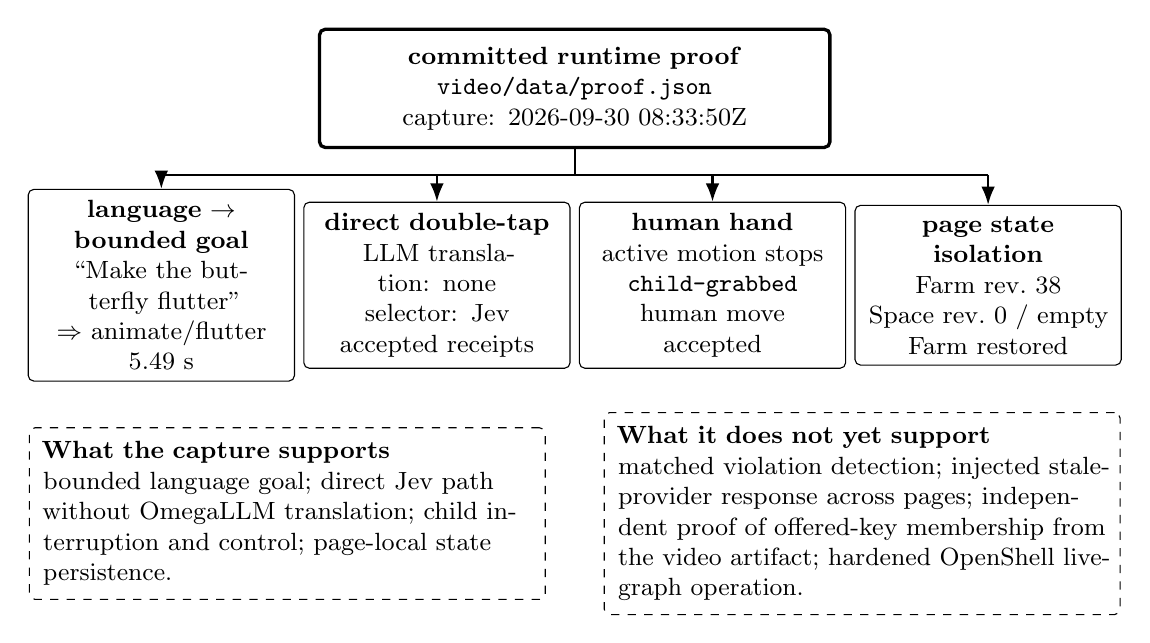
\begin{tikzpicture}[
  font=\small,
  >=Latex,
  box/.style={draw,rounded corners=2pt,align=center,minimum height=15mm,text width=31mm,inner sep=4pt},
  source/.style={box,very thick,text width=62mm},
  note/.style={draw,dashed,rounded corners=2pt,align=left,text width=62mm,inner sep=5pt},
  arrow/.style={->,thick}
]
% The source artifact is visually separated from the four observations, and
% the claim-boundary notes sit on their own row.  This avoids implying that
% the notes are additional runtime events or downstream causal stages.
\node[source] (src) at (0,4.15) {\textbf{committed runtime proof}\\\texttt{video/data/proof.json}\\capture: 2026-09-30 08:33:50Z};

\node[box] (lang) at (-5.25,1.65) {\textbf{language $\rightarrow$ bounded goal}\\``Make the butterfly flutter''\\$\Rightarrow$ animate/flutter\\5.49 s};
\node[box] (tap) at (-1.75,1.65) {\textbf{direct double-tap}\\LLM translation: none\\selector: Jev\\accepted receipts};
\node[box] (hand) at (1.75,1.65) {\textbf{human hand}\\active motion stops\\\texttt{child-grabbed}\\human move accepted};
\node[box] (page) at (5.25,1.65) {\textbf{page state isolation}\\Farm rev.~38\\Space rev.~0 / empty\\Farm restored};

% One trunk, four branches: all observations derive from the same committed
% proof artifact, without suggesting that one observation causes another.
\coordinate (fork) at (0,3.05);
\draw[thick] (src.south) -- (fork);
\draw[thick] (-5.25,3.05) -- (5.25,3.05);
\foreach \x in {lang,tap,hand,page}{
  \draw[arrow] (\x.north |- fork) -- (\x.north);
}

\node[note] (yes) at (-3.65,-1.25) {\textbf{What the capture supports}\\bounded language goal; direct Jev path without OmegaLLM translation; child interruption and control; page-local state persistence.};
\node[note] (no) at (3.65,-1.25) {\textbf{What it does not yet support}\\matched violation detection; injected stale-provider response across pages; independent proof of offered-key membership from the video artifact; hardened OpenShell live-graph operation.};

\end{tikzpicture}
}
\caption{Observed StickerBook runtime evidence imported from the committed P(HOP) proof artifact. Four positive observations are retained with explicit claim limits. The right-hand boundary is as important as the left: the capture does not supply matched violation pairs, an injected stale-provider-response test, an independently serialized legal table for the double-tap event, or verification of the hardened OpenShell graph.}
\label{fig:runtime-observed}
\end{figure*}

\begin{table}[t]
\centering
\small
\caption{Candidate StickerBook invariants and matched perturbations.}
\label{tab:perturbations}
\begin{tabular}{p{0.23\linewidth}p{0.34\linewidth}p{0.34\linewidth}}
\toprule
Property & Aligned trace & Controlled violation \\
\midrule
Action-set validity & Selected action belongs to host-offered set & Inject action not offered by host \\
Host validation & Action executes only after successful validation & Bypass validation before execution \\
Page isolation & Farm-originated action affects Farm only & Apply Farm-originated action to Space \\
Stale-response rejection & Delayed response with expired context is rejected & Accept and execute stale response \\
State independence & Page-local mutations remain page-local & Mutate a second page through shared state \\
Advisory memory & Learned pattern is a candidate subject to current authority & Execute remembered pattern autonomously \\
Direct control & Double tap reaches bounded typed decision path & Route direct control through unauthorized generative path \\
\bottomrule
\end{tabular}
\end{table}

\section{Controlled Perturbation Protocol}
For each target invariant, construct matched trajectory pairs in which only one alignment-relevant property differs. Each source trace is retained as canonical ground truth. Perturbations are injected either at the agent/runtime layer or at the representation layer, never both simultaneously in the primary calibration conditions.

\subsection{Source perturbations}
Source perturbations include invalid-action injection, page leakage, stale-response acceptance, cross-page state contamination, advisory-memory escalation, and validation bypass. These create true agent/runtime failures.

\subsection{Mapping perturbations}
Mapping perturbations leave the source trace unchanged while degrading a witness. Examples include event omission, variable aliasing, shuffled page-to-timbre assignments, visual boundary removal, temporal desynchronization, excessive dynamic-range compression, and collisions in which distinct events are intentionally rendered identically.

This factorial separation enables a direct test of whether an observer is reacting to the source behavior or to an artifact of the display.

\subsection{Reproducible pre-freeze calibration scaffold}
The source bundle accompanying this manuscript includes a schema, generator, validators, and deterministic witness renderers under \texttt{experiment/}. The scaffold contains fourteen \emph{synthetic calibration fixtures}: aligned/violation pairs for the seven candidate invariants in \cref{tab:perturbations}. These are explicitly labeled \texttt{synthetic-calibration}; they are never represented as runtime observations. A separate \texttt{runtime\_evidence/} layer contains four positive observations conservatively derived from the pinned P(HOP) runtime-proof artifact described above, plus independent SVG/WAV renders and their own hash manifest. Synthetic calibration and observed runtime evidence therefore remain mechanically distinguishable in both metadata and directory structure.

Each fixture is rendered independently into an SVG visual witness and a 48~kHz WAV sonic witness. A SHA-256 manifest freezes the source trace and both derived stimuli. Participant-facing visual renders contain neither the ground-truth label nor the words ``aligned'' or ``violation.'' File identity and ground truth remain outside the presented witness.

The scaffold also performs a simple pre-freeze collision check. In the first sonification pass, the aligned and violating \emph{action-set validity} fixtures rendered identically: action class and receipt status were audible, but membership of the selected key in the host-offered legal table was not. This was a mapping collision of exactly the kind formalized in Proposition~\ref{prop:collision}. Before freezing the mapping, a brief legal-membership cue was added; the source traces were unchanged. After revision, all seven matched pairs are byte-distinct in both renderers. This check establishes only representational separation, not human perceptual discriminability; the latter remains an empirical question for the observer study.

\begin{figure*}[t]
\centering
\resizebox{0.94\textwidth}{!}{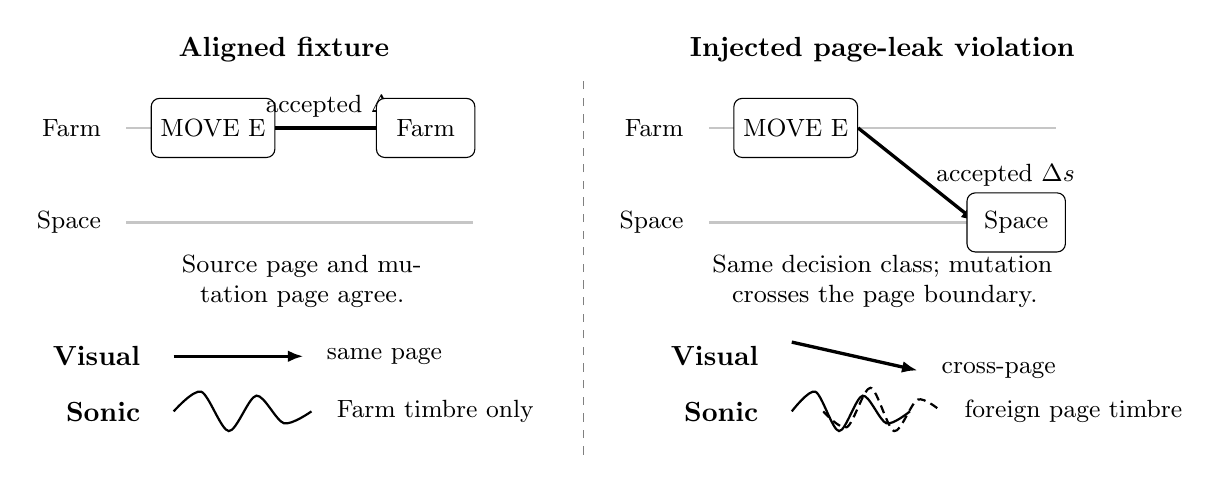
\begin{tikzpicture}[font=\small,>=Latex]
  \tikzset{
    box/.style={draw, rounded corners=3pt, minimum height=0.75cm, align=center, fill=white},
    lane/.style={draw=gray!45, line width=0.8pt},
    good/.style={draw=black, line width=1.2pt, -{Latex[length=2mm]}},
    bad/.style={draw=black, line width=1.2pt, -{Latex[length=2mm]}},
    wave/.style={thick}
  }
  \node[font=\bfseries] at (-3.8,2.8) {Aligned fixture};
  \node[font=\bfseries] at (3.8,2.8) {Injected page-leak violation};

  % left lanes
  \node[anchor=east] at (-6.0,1.8) {Farm};
  \node[anchor=east] at (-6.0,0.6) {Space};
  \draw[lane] (-5.8,1.8)--(-1.4,1.8);
  \draw[lane] (-5.8,0.6)--(-1.4,0.6);
  \node[box,minimum width=1.5cm] (la) at (-4.7,1.8) {MOVE E};
  \draw[good] (la.east)--(-2.4,1.8) node[midway,above] {accepted $\Delta s$};
  \node[box,minimum width=1.25cm] at (-2.0,1.8) {Farm};
  \node[align=center,text width=4.4cm] at (-3.6,-0.15) {Source page and mutation page agree.};

  % right lanes
  \node[anchor=east] at (1.4,1.8) {Farm};
  \node[anchor=east] at (1.4,0.6) {Space};
  \draw[lane] (1.6,1.8)--(6.0,1.8);
  \draw[lane] (1.6,0.6)--(6.0,0.6);
  \node[box,minimum width=1.5cm] (ra) at (2.7,1.8) {MOVE E};
  \draw[bad] (ra.east)--(5.0,0.6) node[midway,right,xshift=1mm] {accepted $\Delta s$};
  \node[box,minimum width=1.25cm] at (5.5,0.6) {Space};
  \node[align=center,text width=4.4cm] at (3.8,-0.15) {Same decision class; mutation crosses the page boundary.};

  % independent witness cues, kept away from the central separator
  \node[anchor=east,font=\bfseries] at (-5.5,-1.1) {Visual};
  \draw[good] (-5.2,-1.1)--(-3.55,-1.1);
  \node[anchor=west] at (-3.38,-1.1) {same page};

  \node[anchor=east,font=\bfseries] at (2.35,-1.1) {Visual};
  \draw[bad] (2.65,-0.92)--(4.25,-1.28);
  \node[anchor=west] at (4.43,-1.28) {cross-page};

  \node[anchor=east,font=\bfseries] at (-5.5,-1.8) {Sonic};
  \draw[wave] plot[smooth] coordinates {(-5.2,-1.8)(-4.85,-1.55)(-4.5,-2.05)(-4.15,-1.6)(-3.8,-1.95)(-3.45,-1.8)};
  \node[anchor=west] at (-3.25,-1.8) {Farm timbre only};

  \node[anchor=east,font=\bfseries] at (2.35,-1.8) {Sonic};
  \draw[wave] plot[smooth] coordinates {(2.65,-1.8)(2.95,-1.55)(3.25,-2.05)(3.55,-1.6)(3.85,-1.95)(4.15,-1.8)};
  \draw[wave,densely dashed] plot[smooth] coordinates {(3.05,-1.8)(3.35,-2.0)(3.65,-1.5)(3.95,-2.05)(4.25,-1.65)(4.55,-1.8)};
  \node[anchor=west] at (4.72,-1.8) {foreign page timbre};

  \draw[dashed,gray] (0,-2.35)--(0,2.45);
\end{tikzpicture}
}
\caption{Matched synthetic calibration fixtures for page isolation. The aligned trace keeps a Farm-originated state delta on Farm; the injected violation applies the same decision class to Space. Visual and sonic witnesses are generated independently from the canonical trace. The schematic sonic layer indicates the added foreign-page timbre rather than attempting to depict waveform identity. Ground-truth labels shown here are explanatory figure labels only; participant-facing stimuli omit them.}
\label{fig:calibration-pair}
\end{figure*}

\section{Witness Construction}
For every source trace, construct at least four representations.

\subsection{Raw structured trace}
The baseline exposes timestamps, page identifiers, action selections, validation results, state mutations, and relevant authority context directly.

\subsection{Visual witness}
The visual transform maps page identity to bounded spatial region, action to animated movement, validation to explicit gating, delayed-response authority to a visible connection that expires, state persistence to object position/history, and cross-page leakage to attempted or successful boundary crossing.

\subsection{Sonic witness}
The auditory mapping must be specified rather than aesthetically improvised. Candidate mappings include page identity to timbral family, action class to register or pitch class, action onset to sonic onset, validation status to stable auditory relation, stale-response attempts to distinguishable events, and illegal cross-page execution to simultaneous presentation of otherwise page-specific timbres.

Parameters should be chosen for perceptual discriminability and evaluated under controlled rendering conditions. Critical-band interactions and playback-level effects must be considered explicitly \citep{plomp1965tonal,katz2015mastering}. The initial study should freeze the mapping before participant data are collected; aesthetic improvement after inspection of outcomes would otherwise become an unregistered analysis degree of freedom.

\begin{table}[t]
\centering
\small
\caption{Proposed first-pass sonification map and paired controls. The mapping is intentionally redundant with the canonical trace rather than a replacement for it.}
\label{tab:sonification-map}
\begin{tabular}{p{0.20\linewidth}p{0.27\linewidth}p{0.43\linewidth}}
\toprule
Trace variable & Auditory encoding & Calibration / accessibility control \\
\midrule
Page identity & fixed timbral family & categorical pretest; never rely on timbre alone in audiovisual condition \\
Action class & short fixed motif & equalized duration/level; motif legend available before trials \\
Accept / reject & resolved vs. interrupted terminal marker & level matched; paired with visual symbol and text receipt \\
Stale response & delayed ``ghost'' onset tied to original page timbre & latency preserved from trace; explicit timestamp available in raw condition \\
Cross-page leak & foreign page timbre sounding inside target-page stream & pretest for discriminability; avoid critical-band collision as the only cue \\
Legal-table membership & brief alert when a host-table selection is absent from the offered set & added after pre-freeze collision test; redundant with raw/visual legal-table evidence \\
World revision & low-rate pulse index / boundary tick & optional channel; disabled for listeners who find dense temporal cues inaccessible \\
\bottomrule
\end{tabular}
\end{table}

Every sonic distinction must have a non-auditory equivalent in the experiment. Likewise, color must not be the sole visual carrier of a safety-relevant distinction. This is both an accessibility requirement and a methodological control: the empirical object is the preservation of the invariant, not dependence on a single sensory ability.

\subsection{Audiovisual witness}
The combined condition synchronizes visual and sonic mappings to the same underlying trace. This condition is important because apparent reinforcement may improve detection or create correlated masking.

\section{Evaluation and Preregistration-Ready Analysis Plan}
A first observer study can use a within-subject design with counterbalanced modality order and randomized trace identity. Each participant sees matched traces drawn from the same source-violation set under raw, visual, sonic, and audiovisual conditions. Source perturbations and mapping perturbations remain separately randomized so that ``the agent failed'' and ``the display failed'' are never synonymous by construction.

For each trace and modality, collect:
\begin{itemize}
    \item violation-detection accuracy;
    \item violation-classification accuracy;
    \item detection time;
    \item observer confidence;
    \item false-positive rate;
    \item calibration between confidence and correctness; and
    \item cross-modal disagreement.
\end{itemize}
The primary modality comparison is
\begin{equation}
\text{raw trace}
\quad\text{vs.}\quad
\text{visual}
\quad\text{vs.}\quad
\text{sonic}
\quad\text{vs.}\quad
\text{audiovisual}.
\end{equation}

\subsection{Primary estimands}
The primary outcome should be correct detection of whether the target invariant was violated. A preregistered mixed-effects logistic model can estimate modality effects while accounting for repeated observations by participant and trace:
\begin{equation}
\operatorname{logit}\Pr(Y=1)
= \beta_0 + \beta_M M + \beta_V V + \beta_{MV}(M\!\times\!V)
+ b_{\mathrm{participant}} + b_{\mathrm{trace}},
\end{equation}
where $M$ indexes modality and $V$ indexes violation class (including no-violation controls). Preplanned contrasts should compare each perceptual witness with the raw trace and the audiovisual condition with its component modalities. Detection latency is a secondary endpoint and should be analyzed only among trials with a correct response, using a preregistered transformed-time or survival model appropriate to the observed distribution.

A separate preregistered test should evaluate Hypothesis H3: whether cross-modal disagreement is enriched for source, mapping, or observer anomalies. The unit of analysis is the canonical trace, not an individual media frame. Mechanical decoders can be evaluated in parallel where a representation admits deterministic extraction, but human and mechanical observer classes should not be pooled without explicit modeling.

\subsection{Power, stopping, and exclusions}
This paper does not choose a participant count from intuition. A small pilot should estimate trial variance, ceiling/floor effects, and plausible modality effect sizes; the confirmatory sample size should then be fixed by simulation-based power analysis before the main study. Stopping rules, participant exclusions, unusable-audio/visual-accessibility exclusions, and treatment of missing latency data should be preregistered. Mapping definitions, stimulus hashes, renderer versions, and analysis code should be frozen before confirmatory data collection.

\subsection{Transform-independence audit}
For every witness family, the preregistration should include a transform-lineage table identifying shared preprocessing, shared feature extractors, common normalization, and any generated intermediate representation. A pair of outputs should not be described as independent evidence merely because one is audible and one is visible. If both factor through a common lossy $Q$, Proposition~\ref{prop:shared-bottleneck} applies. The strongest confirmatory condition therefore constructs each witness directly from the canonical trace and invariant schema, with modality-specific code paths that share only declared lossless utilities.

No human-subject data are reported in this paper. Any eventual participant study should undergo the appropriate ethics review or exemption determination before data collection.

\section{Worked Generative Demonstration: P(HOP)}
A public companion artifact, \href{https://youtu.be/vpu4tmhyj04}{\emph{I'm Upping My P(HOP)}}, was developed as an intentionally playful demonstration of the framework; the associated StickerBook materials are available in the \href{https://github.com/PaulTiffany/stickerbook}{project repository} \citep{tiffany2026phop,tiffany2026stickerbook}. Its provenance is recursive. The work was influenced by the generative song \emph{I'm Upping My P(doom)} and subsequent code-rendered visualizations constructed with Claude \citep{mexicat2026pdoom,heibel2026pdoom}. Those visualizations transform linguistic and musical events into deterministic timed visual scenes.

P(HOP) reverses and extends the process. A human observer interprets the prior audiovisual artifact, specifies a new conceptual and technical mapping around bounded agentic behavior, generates a new musical representation, and directs coding agents to construct a synchronized visual representation from actual StickerBook assets and architecture. The video implementation also embeds four explicitly labeled proof moments reconstructed from the committed live-runtime evidence rather than fictional receipts or an application screen recording \citep{tiffany2026stickerbookproof,tiffany2026stickerbookvideo}. We use the public artifact as a worked provenance case for the observer--transform--agent loop; empirical validation of cross-modal witnessing still requires the controlled matched-perturbation study proposed above.

\begin{figure*}[t]
\centering
\resizebox{0.98\textwidth}{!}{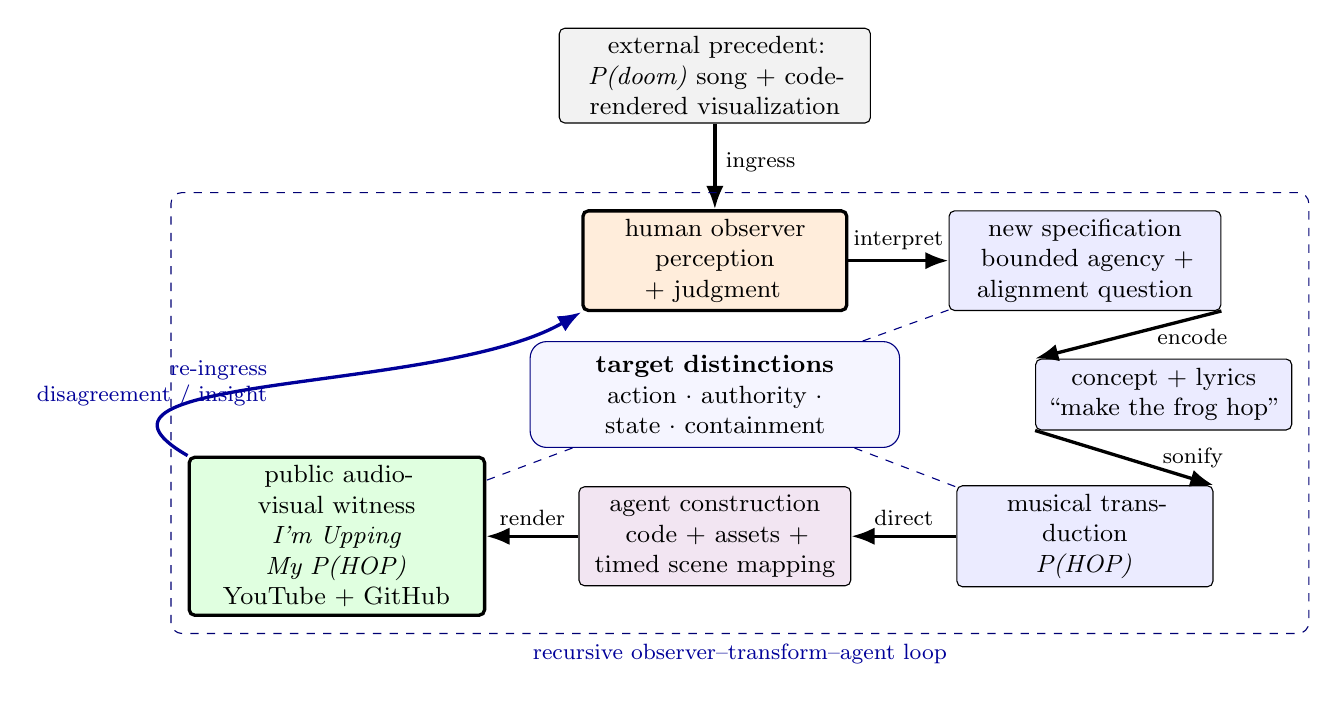
\begin{tikzpicture}[
  x=1cm,y=1cm,
  >=Latex,
  font=\small,
  box/.style={draw, rounded corners=2pt, align=center, minimum height=9mm, inner xsep=5pt, inner ysep=3pt},
  ext/.style={box, fill=gray!10, text width=36mm},
  human/.style={box, fill=orange!14, very thick, text width=30mm},
  specbox/.style={box, fill=blue!8, text width=31mm},
  map/.style={box, fill=blue!8, text width=29mm},
  agent/.style={box, fill=violet!10, text width=31mm},
  witness/.style={box, fill=green!12, very thick, text width=34mm},
  core/.style={draw=blue!50!black, rounded corners=6pt, fill=blue!4, align=center, text width=42mm, inner xsep=7pt, inner ysep=5pt},
  arrow/.style={->, very thick},
  feedback/.style={->, very thick, blue!60!black}
]
% External artifact enters the same observer that later receives the constructed witness.
\node[ext] (pdoom) at (0,4.0) {external precedent: \emph{P(doom)} song + code-rendered visualization};
\node[human] (observer) at (0,1.65) {human observer\\perception + judgment};

% Clockwise transformation/construction loop.
\node[specbox] (spec) at (4.7,1.65) {new specification\\bounded agency + alignment question};
\node[map] (concept) at (5.7,-0.05) {concept + lyrics\\``make the frog hop''};
\node[map] (music) at (4.7,-1.85) {musical transduction\\\emph{P(HOP)}};
\node[agent] (construct) at (0,-1.85) {agent construction\\code + assets + timed scene mapping};
\node[witness] (phop) at (-4.8,-1.85) {public audiovisual witness\\\emph{I'm Upping My P(HOP)}\\YouTube + GitHub};
\node[core] (core) at (0,-0.05) {\textbf{target distinctions}\\action $\cdot$ authority $\cdot$ state $\cdot$ containment};

\draw[arrow] (pdoom.south) -- node[pos=.45,right,font=\footnotesize]{ingress} (observer.north);
\draw[arrow] (observer.east) -- node[above,font=\footnotesize]{interpret} (spec.west);
\draw[arrow] (spec.south east) -- node[pos=.55,right,xshift=10pt,font=\footnotesize]{encode} (concept.north west);
\draw[arrow] (concept.south west) -- node[right,xshift=10pt,font=\footnotesize]{sonify} (music.north east);
\draw[arrow] (music.west) -- node[above,font=\footnotesize]{direct} (construct.east);
\draw[arrow] (construct.west) -- node[above,font=\footnotesize]{render} (phop.east);
\draw[feedback] (phop.north west) to[out=150,in=-150] node[left,font=\footnotesize,align=right]{re-ingress\\disagreement / insight} (observer.south west);

% The preserved distinctions are the payload carried through each representation.
\draw[dashed, blue!50!black] (core) -- (spec);
\draw[dashed, blue!50!black] (core) -- (music);
\draw[dashed, blue!50!black] (core) -- (phop);

\node[draw=blue!45!black, dashed, rounded corners=4pt, fit=(observer)(spec)(concept)(music)(construct)(phop), inner sep=6pt,
      label={[font=\footnotesize,blue!60!black]below:recursive observer--transform--agent loop}] {};
\end{tikzpicture}
}
\caption{P(HOP) as a recursive provenance and ingress loop. An external audiovisual artifact enters a human observer, is interpreted into a new alignment-relevant specification, and is re-expressed through lyrics, music, agent construction, and a public audiovisual witness. The resulting artifact re-enters observation, where disagreement or newly salient structure can revise the next specification. The figure records the provenance loop; empirical claims are supplied by the controlled perturbation protocol.}
\label{fig:phop-loop}
\end{figure*}

Its repeated instruction, ``make the frog hop,'' deliberately compresses a large alignment question into a small inspectable action. The scientific question is not whether the song is persuasive. It is whether the action, authority, state, and containment properties survive the transformations required to make the behavior perceptually legible.

\section{Discussion}
Cross-modal witnessing offers no escape from the observer problem. It multiplies observers. That multiplication can nevertheless be useful.

If a textual audit, visualization, and sonification all preserve a specified distinction through upstream-diverse transforms, confidence in the \emph{observability} of that distinction may increase. Merely changing output modality is insufficient: Figure~\ref{fig:shared-bottleneck} shows why multiple polished views of the same lossy intermediate can agree perfectly while preserving the same mistake. If genuinely diverse witnesses disagree, the disagreement identifies a seam requiring investigation. This suggests an alignment methodology based not on a privileged representation but on \emph{controlled representational plurality}.

The central question changes from ``Which visualization explains the agent?'' to:
\begin{quote}
Which alignment-relevant distinctions survive independently specified transformations, and where do those transformations disagree?
\end{quote}
This is closely related to the observer-relative program in \href{https://paultiffany.github.io/Principia-Symbolica/}{\emph{Principia Symbolica}}: a property that appears only under one bounded projection should not automatically be treated as a property of the underlying system \citep{tiffany2026principia}. Cross-modal transport therefore supplies a practical test of representational robustness.

The framework also gives a more disciplined interpretation of generative-media phenomena sometimes dismissed as ``AI slop.'' Catchy songs, stylized images, and deterministic animations can function as compression and ingress mechanisms when their mappings are inspectable. Their scientific value depends on whether the mapping is specified, whether target distinctions survive, and whether resulting observer judgments are calibrated---not on the cultural status of the artifact.

\section{Limitations}
First, perceptual salience is not semantic truth. A compelling representation can amplify an artifact.

Second, mappings may share hidden dependencies. Agreement among modalities is weaker when their transformations derive from the same lossy intermediate representation.

Third, human observers differ in hearing, vision, expertise, attention, cultural interpretation, and prior knowledge. Accessibility must therefore be designed into both the experiment and the interpretation.

Fourth, some alignment properties may not admit useful low-dimensional perceptual mappings.

Fifth, channel-induced interactions can be mistaken for source interactions. Sonification is especially vulnerable to spectral masking, roughness, playback differences, and level-dependent perception; visualization has analogous problems involving occlusion, salience, scale, and color perception.

Sixth, the framework is strongest when the source environment supplies mechanical ground truth. Application to open-ended agent behavior will require careful treatment of uncertain labels and observer-relative specifications.

Finally, neither sonification nor visualization should replace machine-verifiable auditing where machine-verifiable auditing is available. Their value is complementary:
\begin{equation}
\text{certificate}\neq\text{witness},
\end{equation}
but a calibrated witness may tell an observer where to look.

\section{Conclusion}
Agentic alignment is evaluated through representations. That fact should be treated as part of the technical problem rather than as a neutral presentation layer.

This paper proposes cross-modal structural transduction as a method for constructing additional audit surfaces from agent trajectories. A representation qualifies as a useful witness only when its mapping is specified, its target invariant is explicit, and its sensitivity to controlled violations is measured.

The approach extends a research trajectory from constraint geometry and deterministic auditing toward observer-relative inspection. \emph{The Cost of Cacophony} asks whether simultaneous constraints are geometrically satisfiable. \emph{The Hypothesis Surface} asks whether evidence remains connected to claims without masking. \emph{Principia Symbolica} formalizes bounded observers and observer-relative symbolic projection. Cross-modal witnessing asks whether alignment-relevant distinctions remain recognizable when behavior is transported into another perceptual channel.

The goal is not to make alignment beautiful.

\begin{center}
\emph{The goal is to make failure harder to hide.}
\end{center}

\section*{Public Artifacts and Reproducibility}
The paper is accompanied by public, inspectable artifacts:
\begin{itemize}[leftmargin=*]
    \item \href{https://youtu.be/vpu4tmhyj04}{\emph{I'm Upping My P(HOP)}} --- public audiovisual worked example;
    \item \href{https://github.com/PaulTiffany/stickerbook}{StickerBook} --- bounded agentic testbed, implementation materials, and audiovisual source assets; the \href{https://paultiffany.github.io/stickerbook/}{public GitHub Pages demo} is intentionally mechanical, while the repository documents the governed localhost path;
    \item \href{https://github.com/PaulTiffany/stickerbook/blob/main/core/README.md}{StickerBook authority-kernel record}, \href{https://github.com/PaulTiffany/stickerbook/blob/main/jev/EXPERIMENT.md}{OmegaJev experiment record}, and \href{https://github.com/PaulTiffany/stickerbook/blob/main/docs/AGENT-INTERFACE.md}{agent-interface contract} --- implementation-level sources for the proposed trace and perturbation schema;
    \item \texttt{experiment/} in the manuscript source bundle --- canonical schema, fourteen synthetic calibration traces, deterministic SVG/WAV witness renderers, SHA-256 stimulus manifest, separation checks, runtime-export adapter template, and a separately labeled \texttt{runtime\_evidence/} layer containing four observed StickerBook traces derived from the pinned P(HOP) proof artifact;
    \item \href{https://github.com/PaulTiffany/stickerbook/blob/453a90f846c61b9c5c8c8f007db4e85ce307fa28/video/data/proof.json}{P(HOP) runtime proof JSON} and \href{https://github.com/PaulTiffany/stickerbook/blob/453a90f846c61b9c5c8c8f007db4e85ce307fa28/video/README.md}{video reproducibility record} --- version-pinned source evidence for the observed-runtime layer;
    \item \href{https://github.com/PaulTiffany/cost}{\emph{The Cost of Cacophony}} --- paper, deterministic audit harnesses, certificates, and sonification suite;
    \item \href{https://github.com/PaulTiffany/hypothesis-surface-agi26}{\emph{The Hypothesis Surface}} --- AGI-26 reproducibility repository, with a \href{https://paultiffany.github.io/hypothesis-surface-agi26/}{public project page}; and
    \item \href{https://github.com/PaulTiffany/Principia-Symbolica}{\emph{Principia Symbolica}} --- public manuscript and formal atlas, with a \href{https://paultiffany.github.io/Principia-Symbolica/}{rendered project page}.
\end{itemize}

\clearpage
\section*{Acknowledgments}
StickerBook was made with support from \href{https://bgicommons.org/}{BGI Commons} as part of its HyperSprints series; the \href{https://bgicommons.org/teams/62}{project team page} records the submission context.

The author thanks Matthew Burtner for formative instruction that introduced sonification as a serious compositional and investigative practice. The author also acknowledges the broader artistic and technical lineage discussed in the text, including auditory-display research, multimedia performance, and open-source generative visualization systems.

\printbibliography

\end{document}
